%%%%%%%%%%%%%%%%%%%%%%%%%%%%%%%%%%%%%%%%%
% Homework Assignment Article
% LaTeX Template
% Version 1.3.1 (ECL) (08/08/17)
%
% This template has been downloaded from:
% Overleaf
%
% Original author:
% Victor Zimmermann (zimmermann@cl.uni-heidelberg.de)
%
% License:
% CC BY-SA 4.0 (https://creativecommons.org/licenses/by-sa/4.0/)
%
%%%%%%%%%%%%%%%%%%%%%%%%%%%%%%%%%%%%%%%%%

%----------------------------------------------------------------------------------------

\documentclass[a4paper]{article} % Uses article class in A4 format

%----------------------------------------------------------------------------------------
%	FORMATTING
%----------------------------------------------------------------------------------------

\addtolength{\hoffset}{-2.25cm}
\addtolength{\textwidth}{4.5cm}
\addtolength{\voffset}{-3.25cm}
\addtolength{\textheight}{5cm}
\setlength{\parskip}{0pt}
\setlength{\parindent}{0in}

%----------------------------------------------------------------------------------------
%	PACKAGES AND OTHER DOCUMENT CONFIGURATIONS
%----------------------------------------------------------------------------------------

\usepackage{blindtext} % Package to generate dummy text
% \usepackage[style=numeric,sorting=none]{biblatex}
\usepackage{charter} % Use the Charter font
\usepackage[utf8]{inputenc} % Use UTF-8 encoding
\usepackage{microtype} % Slightly tweak font spacing for aesthetics

\usepackage[english]{babel} % Language hyphenation and typographical rules

\usepackage{amsthm, amsmath, amssymb} % Mathematical typesetting
\usepackage{float} % Improved interface for floating objects
\usepackage[final, colorlinks = true, 
            linkcolor = black, 
            citecolor = black]{hyperref} % For hyperlinks in the PDF
\usepackage{graphicx, multicol} % Enhanced support for graphics
\usepackage{xcolor} % Driver-independent color extensions
\usepackage{marvosym, wasysym} % More symbols
\usepackage{rotating} % Rotation tools
\usepackage{censor} % Facilities for controlling restricted text
\usepackage{listings, style/lstlisting} % Environment for non-formatted code, !uses style file!
\usepackage{pseudocode} % Environment for specifying algorithms in a natural way
\usepackage{style/avm} % Environment for f-structures, !uses style file!
\usepackage{booktabs} % Enhances quality of tables
\usepackage{hyperref}

\usepackage{tikz-qtree} % Easy tree drawing tool
\tikzset{every tree node/.style={align=center,anchor=north},
         level distance=2cm} % Configuration for q-trees
\usepackage{style/btree} % Configuration for b-trees and b+-trees, !uses style file!

% \usepackage[backend=biber,style=numeric,
            % sorting=nyt]{biblatex} % Complete reimplementation of bibliographic facilities
% \addbibresource{ecl.bib}
\usepackage{csquotes} % Context sensitive quotation facilities

\usepackage[yyyymmdd]{datetime} % Uses YEAR-MONTH-DAY format for dates
\renewcommand{\dateseparator}{-} % Sets dateseparator to '-'

\usepackage{fancyhdr} % Headers and footers
\pagestyle{fancy} % All pages have headers and footers
\fancyhead{}\renewcommand{\headrulewidth}{0pt} % Blank out the default header
\fancyfoot[L]{School of Computing, Macquarie University} % Custom footer text
\fancyfoot[C]{} % Custom footer text
\fancyfoot[R]{\thepage} % Custom footer text

\usepackage{comment}
\newcommand{\note}[1]{\marginpar{\scriptsize \textcolor{red}{#1}}} % Enables comments in red on margin

%----------------------------------------------------------------------------------------

\begin{document}

%----------------------------------------------------------------------------------------
%	TITLE SECTION
%----------------------------------------------------------------------------------------

\title{COMP3100 project report} % Article title
\fancyhead[C]{}
\hrule \medskip % Upper rule
\begin{minipage}{1\textwidth} % Center of title section
\centering 
\large % Title text size
Project report: Stage 2\\ % Assignment title and number
COMP3100 Distributed Systems, S1, 2023\\
\normalsize % Subtitle text size
SID: 46463100, Name: Hasham Masood
%%%%\\ % Assignment subtitle
\end{minipage}
\medskip\hrule % Lower rule
\bigskip

%----------------------------------------------------------------------------------------
%	ARTICLE CONTENTS
%----------------------------------------------------------------------------------------
\section{Introduction}
This paper was written with the objective of creating a scheduling algorithm that presents an efficient average turnaround time. This goal is to be achieved without neglecting performance metrics such as total rental cost and resource utilisation. The client that I have designed was made to work alongside \textbf{\textls{ds-server}} which may be found {\emph{ds-sim repository}}\cite{MQGithub}. In stage 1, we utilised \textit{Largest Round Robin} scheduling algorithm which maximised resource utilisation and reduced total rental costs. Despite this result, it had an inherent weakness in presenting sound turnaround times. This metric is concerned with monitoring the time required to schedule and complete a job. In this stage, I have designed a customised First-Fit Algorithm which sends \textit{Gets Avail} and conditionally sends a \textit{Gets Capable} request to the server. My own personal GitHub repository with my client may be found at the following \href{https://www.google.com}{GitHub Repository}\cite{MyGithub}. The decision to choose First-Fit was made when observing the baseline algorithm's performance in the Python Test Suites provided in the Week 11 workshop. In the following sections we will go further in-depth with why it is the effective choice.

\section{Section 2: Problem Definition}
\label{sec:section2}
As eluded to in the previous section, when experimenting with the baseline algorithms it is rather apparent that \textbf{\textls{First-Fit}} ('FF') and \textbf{\textls{Best-Fit}} ('BF') are by far the most efficient algorithms that yield low turnaround times whilst maintaining an agreeable result in other metrics. The initial step in testing resulted in comparing the Results of LRR against these baseline algorithms. I have included a brief overview of these findings in the table below. For this reason, I opted to select FF as my algorithm of choice. The thought behind this was that I would be able to change some details that may yield some performance gains. After successfully implementing First-Fit as may be seen in the commit history of the repository I would tweak the algorithm. Before we discuss this change, let us ensure we have a grounded understanding of how First-Fit scheduling works. FF schedules jobs by sorting through the list of provided servers and finding the first server that has the requirements to satiate the job's requirements (i.e., core count). If it is unable to do so, it will select the first capable server regardless of its availability. My logic changes this so that it sorts through the list of Available servers if there are no available servers it then invokes the use of Gets Capable following the identical logic. This theory and its successful implementation propel the vision I have for this project. In the table below, we may view the deficiencies of our now-dated algorithm against the baseline algorithms.   

\begin{table}[h!]
    \centering
    \begin{tabular}{|c|c|c|c|c|c|}
    \hline
        FF & BF & FFQ & BFQ & WFQ & LRR\\
    \hline
    2400 & 2397 & 2802 & 2630& 6880 & 7729\\\hline
    388 & 373  & 813 & 698 & 3804 & 4930\\\hline
    654 & 653 & 893 & 831 & 4576 & 4045\\\hline
    61 & 60 & 106 & 100 & 677 & 212\\\hline
    3123 & 4674 & 6536 & 6666& 23972& 126721\\\hline
    \end{tabular}
    \label{tab:my_label}
    \caption{Baseline Algorithm Turnaround Times}
\end{table}


\section{Section 3: Algorithm Description}
\label{sec:section3}
In this section, we will closely observe the actions of our customised algorithm through the use of a predetermined configuration file, and the \textbf{\textls{ds-viz}} utility to visualise the process of the scheduling operation. The config file that I have selected is that which was provided to us in Week 9's Workshop, \textit{ds-config01--wk9}. This config includes the presence of three servers tiny, small, and medium. To effectively describe our algorithm, we will present the results of this config file in a concise manner to further the reader's comprehension. After initiating the handshake, the server sends JOBN which is a normal job that requires to be scheduled. Our algorithm reads the core, memory, and disk requirement of this job. It proceeds to iterate through the list of available servers finding the first server that has sufficient or greater cores to house the scheduling of the job. Using the configuration file below, our first job, requires a server with at least 1 core available. The server that satiates this requirement is server tiny. Therefore, JOBID 0 is scheduled for this server. The second job also requires one core, now that tiny is currently occupied it no longer displays via the Gets Avail request. The first server available with its (the job) requirement is the server small which has 2 cores available. Thus, the JOBID 1 is scheduled to small. As we progress, there are eventually no servers available to accommodate the given job. In this instance, we send Gets Capable and schedule the job to the first capable server with the core requirement identical to the default baseline equivalent of our algorithm. It is at this stage we may observe the inadequacies of First-Fit. By scheduling exclusively to capable servers, the client does not take into consideration if the given server is immediately available to schedule the job. For this reason, jobs may find themselves in lengthy queues more apparent in larger-scale models. The customised algorithm excels in this situation which we will explore in later sections within this paper. Where we will check our code against the Python test suits introduced to us in Week 11's workshop.

\begin{verbatim}
<!--  generated by: Y. C. Lee  -->
<config randomSeed="65535">
<servers>
<server type="tiny" limit="1" bootupTime="40" hourlyRate="0.4" cores="1" memory="4000" disk="32000"/>
<server type="small" limit="1" bootupTime="40" hourlyRate="0.4" cores="2" memory="8000" disk="64000"/>
<server type="medium" limit="1" bootupTime="60" hourlyRate="0.8" cores="4" memory="16000" disk="128000"/>
</servers>
\end{verbatim}

\subsection{Section 3.1: Visualisation}

At this stage of the paper, the reader should have a sound understanding of the proccesses involved with both First-Fit and my customised implementation of it. We may present a visualisation based upon this knowledge utilising the \textbf{\textls{ds-viz}} utility. We will present a snippet belonging to the default baseline algorithm to check against our own. 

\begin{figure}[h]
    \centering
    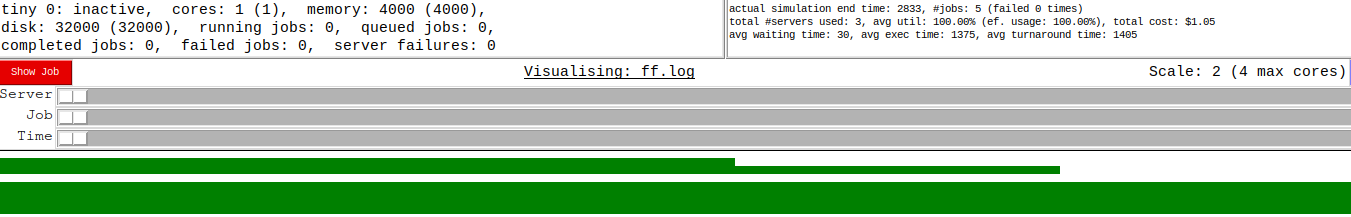
\includegraphics[width=1\textwidth]{images/ffds.png}
    \caption{First-Fit Visualised}
    \label{fig:my_label}
\end{figure}

\begin{figure}[h]
    \centering
    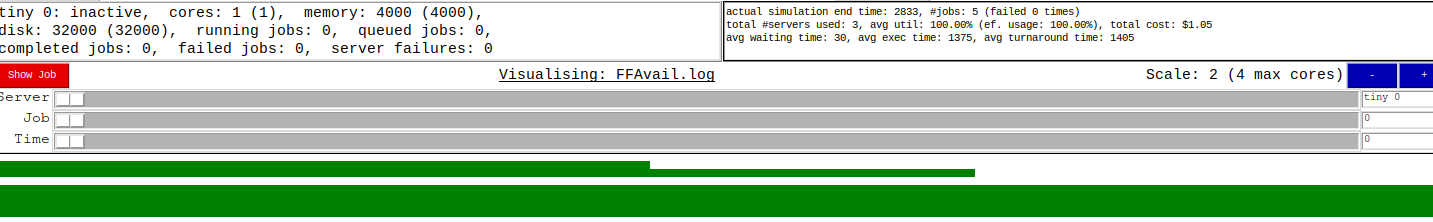
\includegraphics[width=1\textwidth]{images/ffcustom.png}
    \caption{Customised Algorithm Visualised}
    \label{fig:my_label}
\end{figure}

I would suggest the reader not gaze too deeply in search of a striking difference. There is actually no visible difference between the two algorithms. The completion statement read identically between the two. This is partly due to the aforementioned case of having configuration files that have few servers and jobs. This is a design principle of FF meaning both servers will excel at finding the correct server if the amount of data to parse is small. The use of Gets Avail is more powerful when there is a greater list of servers available. In our evaluation section, we will further elaborate on how to make more meaningful changes to our code to improve turnaround times.

\section{Section 4: Implementation}
In this section, we will explain the logic and provide information associated with the data structure(s) used in our code. Let us briefly refresh our knowledge of how our client functions. For a more in-depth understanding, please refer to the Stage 1 Report. Our Client initiates a handshake with the ds-server. This involves the client sending 'HELO', 'AUTH', and 'REDY' after this initial communication the server sends us the job information (or JOBN). This leads to ur while loop which runs continuously until the server sends "NONE" signifying that there are no more jobs to be scheduled. This then presents us with the following code:

\begin{verbatim}
 if (serverResponse.contains("JOBN")) {
            String[] jobData = serverResponse.split(" ");
            int jobCore = Integer.valueOf(jobData[4]);
            int jobMemory = Integer.valueOf(jobData[5]);
            int jobDisk = Integer.valueOf(jobData[6]);
            clientSend("GETS Avail " + jobCore + " " + jobMemory + " " + jobDisk);
            String test = clientRead();
\end{verbatim}

In this section, we split the server's response which is the information pertaining to the job. We utilise the 'Integer.valueOf(string)' to convert the string to an integer. So that we may access the core, memory, and disk requirement of the job. We then send "Gets Avail" with the information we gathered from the JOBN string and store that response in a variable. We then split this response which tells us the number of servers that are available for our chosen GETS message.

\begin{verbatim}
 String[] serverInfo = test.split(" ");
 int nrecs = Integer.valueOf(serverInfo[1]);
\end{verbatim}

The next important component of our code is the condition in which we decide whether we should send Gets Capable, if the prior code results in the server sending "Data 0 X". We know that there are no available servers to house the job. Then we send "OK" so that we may send Gets Capable and parse that information into our for loop that follows the if condition.
\begin{verbatim}
if (nrecs == 0){
              clientSend("OK");
              clientRead();
              clientSend("GETS Capable " + jobCore + " " + jobMemory + " " + jobDisk);
              test = clientRead();
              serverInfo = test.split(" ");
              nrecs = Integer.valueOf(serverInfo[1]);
            }
\end{verbatim}

This leads us to our for loop which has the conditions for the First-Fit Algorithm. We begin by using a Boolean Flag which ensures that the server reads all the responses before returning a False value. We then store the first server that is able to accommodate the job which is used if the condition after is not met. The loop then ensures that the server has enough or more cores to be able to execute the job. This is where our Boolean flag is set to true if a server that can accommodate the job is found. If no server is found it is instead sent to the first capable server.
\begin{verbatim}
     boolean serverLocatedFlag = false;

         for (int i = 0; i < nrecs; i++) {
            String currentServerData = dis.readLine();
            String[] serverDataArr = currentServerData.split(" ");
            int serverCores = Integer.parseInt(serverDataArr[4]);
            
            if (i == 0) {
            firstServer = currentServerData;
            }
            
            if (serverCores >= jobCore && !serverLocatedFlag) {
                serverData = currentServerData;
                serverLocatedFlag = true;
              }
            }
            if (!serverLocatedFlag) {
              serverData = firstServer;
            }
\end{verbatim}

We then split 'serverData' from the for loop so that we may get the serverType (i.e., small) and the serverID. This is then scheduled to the server. When the server sends "NONE" we are able to QUIT and close the connection.

\section{Section 5: Evaluation}
In evaluating the success of my algorithm I have utilised the Python test suite that was provided to us in Week 11's Workshop. We may observe in the screen capture below that our client was successful in achieving its objective of having a lower average turnaround than the baseline algorithms. A noteworthy observation is that our custom algorithm in some test cases performs almost identically to its FF counter-part. This builds on the idea we discovered when running ds-viz pertaining to the size of the job traffic. Despite this, we may see how incredibly are algorithm performs with larger configuration files. In one instance, it yields a 60.15\% lead. The average turnaround time has decreased from 1867.3 to 1414.13 which translates to a 24.26\% improvement. This turnout is in accordance with our hypothesis as using GETs Avail is allowing jobs to be scheduled a lot faster as the presence of the server on the list means they are ready to commence the job immediately. This is opposed to the inevitable creation of queues when using Gets Capable.Despite this, the algorithm is almost certainly limited in its capacity to differentiate itself from the baseline algorithm when dealing with smaller configuration files. 

\begin{figure}[h]
    \centering
    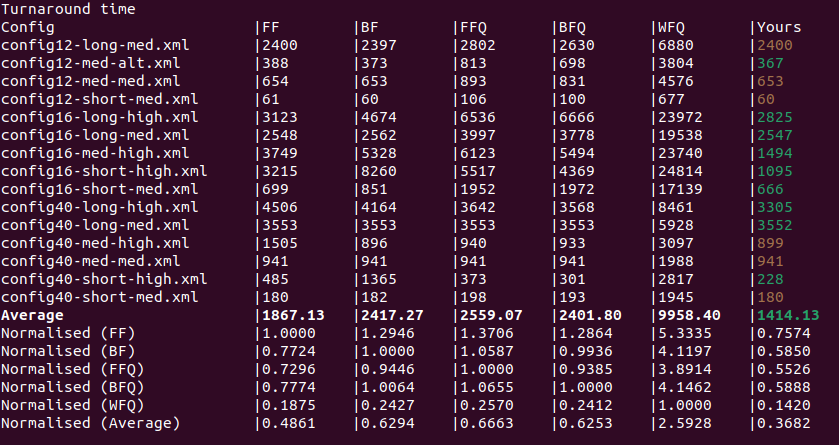
\includegraphics[width=0.6\textwidth]{images/TURNAROUND.png}
    \caption{Turnaround Time Measurement}
    \label{fig:my_label}
\end{figure}

As discussed, the performance whilst maintaining a noticeably lower average is still limited by the weaknesses of the parent algorithm. There are several instances visible above where the results are identical or quite alike. Note config12-long-med as one clear example of this. This may also be observed below in terms of Resource Utilisation and Total Rental Cost.

\begin{figure}[h]
    \centering
    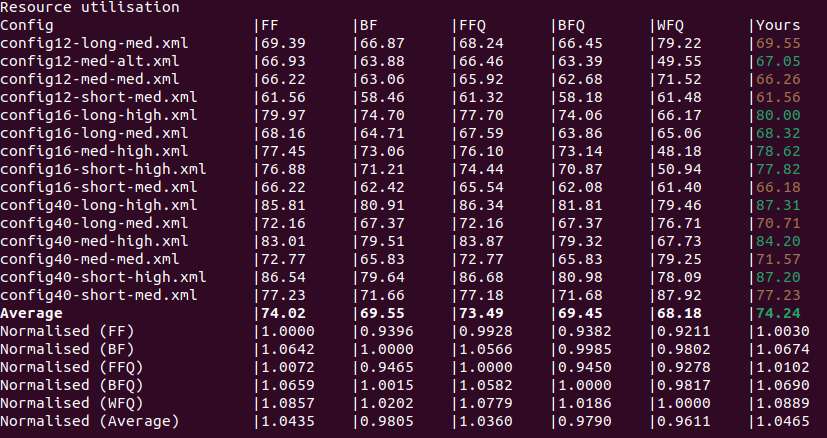
\includegraphics[width=0.6\textwidth]{images/resource util.png}
    \caption{Resource Utilisation Measurement}
    \label{fig:my_label}
\end{figure}

\begin{figure}[h]
    \centering
    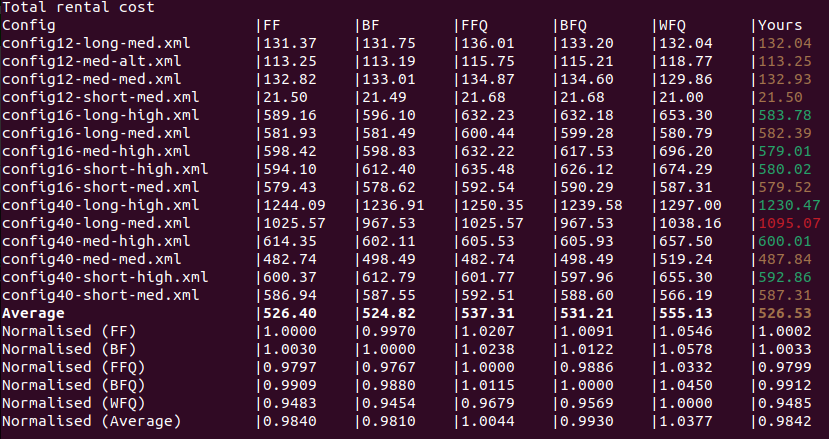
\includegraphics[width=0.6\textwidth]{images/total rental cost.png}
    \caption{Total Rental Cost Measurement}
    \label{fig:my_label}
\end{figure}\newpage

Let us momentarily touch base with the results of the Resource Utilisation and Total Rental Cost metric. To begin with the former, our resource utilisation was marginally greater than FF by a measurement of 0.22\% whilst outperforming WFQ by 6.06\%. It is evident that is a recurring trend to see the difference to be marginal between our algorithm and that of First Fit. When exploring the Total Rental Cost our program is actually confined to the orange colour. As the best average belongs to the Best Fit Algorithm. This is the only performance metric that our algorithm is bested in. 


\section{Section 6: Conclusion}
In conclusion, we may observe that our custom First-Fit algorithm is marginally superior to the baseline algorithms prescribed to this assessment. It is evident that this algorithm's efficiency is entirely based upon two factors. It is reliant on a large number of servers and jobs. This is because its scheduling capacity using Gets Avail is able to find servers that are able to take the job on immediately as opposed to servers that require more time before they can begin completing the job. Despite this, even if the number of jobs and servers were less the algorithm may only work as well as the standard version of First Fit which is not entirely bad as FF is one of the most efficient of the baseline algorithm. I think that if we were to use any other metric to further reduce these turnaround times might be to pay attention to the number of jobs that are currently waiting or running and scheduling on that basis. This may result in more efficient utilisation of the assets of the server.


%----------------------------------------------------------------------------------------
%	REFERENCE LIST
%----------------------------------------------------------------------------------------
\bibliographystyle{ieeetr}
\bibliography{comp3100project}
% \printbibliography

%----------------------------------------------------------------------------------------

\end{document}
